\documentclass[runningheads]{llncs}

\usepackage[T1]{fontenc}
\usepackage{graphicx}
\usepackage{booktabs}
\usepackage{multirow}
\usepackage{array}
\usepackage{amsmath}
\usepackage{url}
\usepackage[hidelinks]{hyperref}
\emergencystretch=3em

\title{ByteBridge: Diagnosing the Limits of Byte Input Adapters for Frozen Tokenizer-Based Language Models}
\titlerunning{ByteBridge}

\author{Anonymous Authors}
\authorrunning{Anonymous Authors}
\institute{Paper under double-anonymous review}

\newcommand{\bb}{ByteBridge}
\newcommand{\qwen}{Qwen2.5-0.5B}
\newcommand{\qwena}{Qwen2.5-1.5B}
\newcommand{\tinyllama}{TinyLlama-1.1B-Chat}
\newcommand{\loss}{\mathcal{L}}
\newcommand{\cratio}{\mathrm{clean\ retention}}

\begin{document}
\maketitle

\begin{abstract}
Subword tokenization is a strong default for language models, but it also creates brittle input behavior on typos, Unicode text, code, paths, and other unusual strings. Byte-level models avoid these input units when they are trained from scratch, but many useful language models are already trained with fixed tokenizers. This paper asks whether such a frozen tokenizer-based model can read byte input through only a small external adapter. We study this question with \bb, a diagnostic benchmark and adapter family for frozen Qwen2.5 and TinyLlama models. The input side is byte-based, while the target side uses each model's native tokenizer so that all systems are scored on the same target tokens. On Qwen2.5, we compare native tokenization with a ladder of byte interfaces: fixed byte patches, embedding distillation, token reconstruction, soft prefixes, and KV-prefix injection. On TinyLlama, we replicate selected later-stage interfaces. The result is mixed. On Qwen2.5, byte adapters consistently help typo-noise inputs, but do not match native tokenization on clean text, Unicode, multilingual text, code, or tokenizer-stress strings. The best \qwen{} adapter improves clean retention from $2.19\times$ to $1.61\times$, but still misses our $1.5\times$ diagnostic threshold and never beats the tokenizer baseline outside typo noise. A \qwena{} replication supports the same negative pattern. On \tinyllama{}, however, all-layer KV-prefix injection reaches $0.63\times$ clean retention averaged over three seeds and beats the tokenizer baseline on clean, typo, and Unicode buckets. This does not imply tokenizer replacement in general: the same adapter still fails on multilingual and tokenizer-stress inputs. These results show that byte adapters can sometimes provide useful input context to a frozen model, but their success is model- and bucket-dependent rather than a general replacement for native tokenization.

\keywords{Tokenization \and Byte-level modeling \and Frozen language models \and Adapter tuning \and Diagnostic study}
\end{abstract}

\section{Introduction}

Subword tokenizers are the front door of most language models. They turn raw text into the discrete units that the model was trained to read. This works well for common text, but it can be brittle. A small typo may change the segmentation. Rare Unicode characters may become many tokens. Code, file paths, long identifiers, and multilingual text may be split in ways that look different from clean English.

Byte-level modeling avoids out-of-vocabulary inputs because every string can be written as bytes. Byte- and character-level models have shown strong robustness and broad coverage when they are trained for this input format from the beginning \cite{alrfou2019character,clark2022canine,gillick2016bytes,kim2016character,tay2022charformer,xue2022byt5,yu2023megabyte}. But many useful language models are not byte models. They were trained with a fixed tokenizer. A tempting shortcut is to keep such a model frozen and train only a small adapter that turns input bytes into continuous vectors the model can use.

This paper tests that shortcut. We ask: \emph{can a small byte adapter give useful input context to a frozen tokenizer-based language model, without badly hurting clean-text performance?} We study this with \bb{}, primarily on Qwen2.5 causal language models \cite{qwen2024technical}, with a selected TinyLlama replication \cite{zhang2024tinyllama}. The language-model backbone, input embedding table, and LM head are always frozen. Only byte-side adapters are trained. The output side still uses each model's native tokenizer, so this is not a fully tokenizer-free language model. It is a test of whether the \emph{input side} of an existing tokenizer-based model can be replaced or augmented by bytes.

There are two plausible outcomes. The optimistic view is that a byte adapter can map UTF-8 bytes into vectors that a frozen model can use. This seems plausible if those vectors are aligned to token embeddings or inserted through prompt- or prefix-tuning interfaces \cite{lester2021prompttuning,li2021prefixtuning}. The pessimistic view is that a tokenizer-based model learns more than a table of token embeddings. It also learns the units, boundaries, positions, and attention patterns created by its tokenizer. A small adapter may not recover all of that structure.

We evaluate these possibilities with a diagnostic ladder. Each step tests one possible reason for failure. We start with fixed-patch byte latents passed through \texttt{inputs\_embeds}. We then test embedding distillation, token reconstruction with fixed, heuristic, and oracle token boundaries, byte-derived soft prefixes, and per-layer KV-prefix injection. The same evaluation suite is reused throughout: clean English, typo noise, Unicode stress, multilingual text, code, and tokenizer-stress strings.

The main result is not a simple success or failure. On Qwen2.5, byte adapters consistently beat the native tokenizer baseline on typo-noise prompts, but every byte adapter is worse on clean text, and the native tokenizer remains better on Unicode, multilingual, code, and tokenizer-stress inputs. Deeper injection helps: all-layer KV-prefix gives the best \qwen{} clean retention, $1.61\times$ the tokenizer baseline. This is progress, but it still misses our $1.5\times$ diagnostic threshold. On \tinyllama{}, the same all-layer KV-prefix interface is much stronger: over three seeds it beats the tokenizer baseline on clean, typo-noise, and Unicode buckets. It still fails badly on multilingual and tokenizer-stress inputs. This cross-family contrast is the central finding: small byte adapters can learn useful byte-side context, but whether they can replace native tokenized input depends strongly on the frozen model and input bucket.

Our contributions are:
\begin{itemize}
    \item We introduce a controlled benchmark and evaluation protocol for input-side byte adapters on frozen tokenizer-based language models, with paired conditional targets and fixed splits.
    \item We provide a phase-by-phase diagnostic study of byte adapters, including input replacement, embedding distillation, token reconstruction, boundary-aware patching, soft prefixes, and KV-prefix injection.
    \item We add three controls for the main story: deterministic preprocessing baselines, fragmentation analysis, and selected replications on \qwena{} and \tinyllama{}.
    \item We report an artifact-backed mixed result: under frozen Qwen2.5, byte adapters improve typo robustness but do not become competitive replacements for native tokenized input; under \tinyllama{}, KV-prefix adapters are stronger but still fail on multilingual and tokenizer-stress inputs.
\end{itemize}

\section{Problem Setting}

Let $M$ be a pretrained causal language model with tokenizer $T$, input embedding matrix $E$, transformer $F$ \cite{vaswani2017attention}, and LM head $H$. In all experiments, $E$, $F$, and $H$ are frozen. Given an input string $x$ and target string $y$, the native tokenizer baseline computes
\begin{equation}
    \loss_{\mathrm{tok}}(x,y) = - \sum_t \log p_M(y_t \mid T(x), y_{<t}),
\end{equation}
where $y_t$ are target tokens under the model's tokenizer. Byte variants replace or augment the conditioning on $x$ with continuous states $A(b(x))$. Here $b(x)$ is the UTF-8 byte sequence and $A$ is the trainable adapter. The target side remains tokenized. This keeps the comparison fair: every system is scored on the same target tokens.

This paired conditional setup is important. Comparisons can be misleading if one system is scored on bytes and another on tokens, or if noisy inputs change the supervised target. We avoid that problem by keeping $y$ fixed. For noisy examples, $x$ is the perturbed string and $y$ is the clean target suffix. Loss is computed only over target tokens, not over byte-prefix or adapter positions.

The main metric is per-bucket target-token loss. We also save perplexity in the experiment artifacts, but focus on loss because stress-bucket perplexities can be very large. To measure clean-text degradation, we use
\begin{equation}
    \cratio(A) = \frac{\loss_A(\mathrm{clean})}{\loss_{\mathrm{tok}}(\mathrm{clean})}.
\end{equation}
Before running the diagnostic ladder, we set two practical thresholds: adapters with at most 50\% higher clean loss than the tokenizer baseline are treated as diagnostically promising ($\cratio \leq 1.5$), and adapters with at most 20\% higher clean loss are treated as strong ($\cratio \leq 1.2$). These are not universal thresholds. They are guardrails that prevent us from calling a byte interface useful when it only wins narrow stress cases by sacrificing clean text.

All reported runs keep the language model and LM head frozen. We record the number of trainable LM parameters and a checksum delta over frozen model tensors. Both must remain zero for a run to be valid.

\section{Benchmark and Metrics}

We construct a small, reproducible suite that stresses tokenizer-unfriendly inputs while remaining feasible in a single-GPU setting. The train, validation, and test manifests are fixed after construction and reused across all phases. Each record contains an identifier, bucket, input text, target text, source, perturbation metadata, seed, and clean-example identifier where applicable. Test examples are never used for training.

The test buckets are:
\begin{itemize}
    \item \textbf{Clean English}: short natural-language, Wikipedia-like, instruction-like, and QA-like snippets.
    \item \textbf{Typo noise}: clean English with random deletion, insertion, substitution, adjacent swaps, repeated characters, whitespace perturbations, and casing noise at light, medium, and heavy levels.
    \item \textbf{Unicode stress}: emoji, accented characters, combining marks, zero-width joiners, full-width characters, mathematical symbols, punctuation variants, and normalized or non-normalized mixtures.
    \item \textbf{Multilingual text}: short Chinese, Japanese, Korean, Arabic, Hindi, Russian, and Latin-script accented examples.
    \item \textbf{Code}: Python, JavaScript, JSON, shell commands, stack traces, regular expressions, SQL, and configuration snippets.
    \item \textbf{Tokenizer-stress strings}: URLs, file paths, package names, UUIDs, base64-like and hexadecimal strings, logs, long identifiers, and mixed separators.
\end{itemize}

Table~\ref{tab:data} gives the split sizes. The benchmark is synthetic and curated. It is not intended to represent natural text frequencies. Its role is to make failure cases visible under controlled conditions.

\begin{table}[t]
\centering
\caption{Fixed splits reused across all phases. The test set contains 500 clean-English examples; 200 examples each for light, medium, and heavy typo noise; 128 Unicode-stress examples; 120 code examples; 120 tokenizer-stress examples; and 80 examples for each multilingual bucket.}
\label{tab:data}
\small
\begin{tabular}{lrrrr}
\toprule
Split & examples & avg. input bytes & avg. input toks & avg. target toks \\
\midrule
train & 5168 & 121.9 & 34.1 & 26.1 \\
validation & 1188 & 99.5 & 30.9 & 25.7 \\
test & 2028 & 100.3 & 30.9 & 25.8 \\
\bottomrule
\end{tabular}
\end{table}

The native tokenizer baseline is the frozen \qwen{} evaluated directly on this paired conditional test set. Its clean-English loss is $0.3089$. This baseline is intentionally strong because it uses the tokenizer and embedding conventions the model saw during pretraining.

\section{ByteBridge Adapter Family}

\subsection{Input-Layer Byte Latents}

The simplest adapter groups bytes into fixed-size patches and maps them into $L$ latent vectors in the language-model hidden dimension. These latents are passed through \texttt{inputs\_embeds} as the prompt representation. This tests the most direct idea: replace tokenized prompt embeddings at the input layer. We train clean-only and noise-augmented variants. The strongest Phase 2 run uses $L=32$ and noise-augmented training for 2000 steps.

\subsection{Embedding Distillation}

One possible failure is that byte latents are not shaped like Qwen token embeddings. To test this, we align byte latents to frozen token embeddings before LM training. We use fixed token-span alignment, where token embeddings are truncated or pooled to $L$ spans, and pooled sequence alignment, where byte and token representations are mean or max pooled. The adapter is then fine-tuned with the same frozen-LM conditional objective.

\subsection{Token Reconstruction and Boundary-Aware Patching}

Embedding MSE may be too weak. The model may need to know which token-like unit a span represents, not just receive a nearby vector. We therefore build a token-byte mapping tool that maps tokenizer tokens to UTF-8 byte spans. For Qwen on this suite, tokenizer offset mapping yields zero unmapped tokens. We test three boundary modes: fixed byte patches, heuristic tokenizer-free boundaries based on UTF-8, script, punctuation, and whitespace changes, and oracle tokenizer-derived byte spans. The oracle mode is a diagnostic upper bound, not a tokenizer-free method.

During reconstruction pretraining, a classifier predicts tokenizer token IDs from byte/span latents. The classifier head is discarded for LM evaluation; only the adapter initializes the frozen-LM conditional training run.

\subsection{Soft Prefix Injection}

Input replacement may be too strict because it forces byte latents to behave like token embeddings at prompt positions. Soft prefix injection uses bytes differently. It compresses input bytes into $P$ learned prefix embeddings, concatenates them before tokenized target embeddings, and computes loss only on target positions:
\begin{equation}
    \mathrm{inputs\_embeds} = [A_{\mathrm{prefix}}(b(x)); E(T(y_{<t}))].
\end{equation}
This keeps native target-side teacher forcing while giving the frozen model byte-derived context.

\subsection{KV-Prefix Injection}

Finally, we test whether bytes must be injected deeper than the input layer. We probe Qwen's \texttt{DynamicCache} API and construct byte-derived key/value tensors with shape $[B, H_{kv}, P, d_h]$ for selected layers. \qwen{} uses 24 layers, hidden size 896, 14 attention heads, 2 key/value heads, and head dimension 64. We test first-4-layer and all-layer injection. For first-$N$ runs, non-injected layers receive zero K/V tensors of the same prefix length to keep cache sequence lengths consistent across layers. This is a diagnostic compromise, not an optimal prefix-tuning design.

\section{Main Results on Qwen2.5-0.5B}

\subsection{Clean Retention Across the Diagnostic Ladder}

Table~\ref{tab:main} summarizes the best representative run from each phase. Lower loss is better. A clean retention of $1.61\times$ means 61\% higher clean loss than the tokenizer baseline. The pattern is consistent: later diagnostics improve some aspects of earlier interfaces, but none approaches native tokenizer conditioning on clean text. The best input-layer reconstruction run reaches $1.84\times$ clean retention. Soft prefixes improve this to $1.76\times$, and all-layer KV-prefix reaches $1.61\times$. All remain above the $1.5\times$ diagnostic threshold.

\begin{table}[t]
\centering
\caption{Representative \qwen{} runs across the diagnostic ladder. ``Typo L/M/H'' denotes the light, medium, and heavy typo-noise buckets. No byte-interface run beats the tokenizer baseline outside typo noise.}
\label{tab:main}
\small
\begin{tabular}{llrrl}
\toprule
Stage & representative run & clean loss & clean retention & wins \\
\midrule
Tokenizer & native Qwen tokenizer & 0.3089 & 1.00 & -- \\
Phase 2 & fixed input, noise, $L=32$ & 0.6770 & 2.19 & typo L/M/H \\
Phase 3 & distill then LM, $L=32$ & 0.6863 & 2.22 & typo L/M/H \\
Phase 4 & fixed recon then LM & 0.5669 & 1.84 & typo L/M/H \\
Phase 5 & soft prefix, $P=64$ & 0.5441 & 1.76 & typo L/M/H \\
Phase 6 & KV prefix, $P=32$, all layers & 0.4985 & 1.61 & typo L/M/H \\
\bottomrule
\end{tabular}
\end{table}

Figure~\ref{fig:qwen-ladder} shows the same clean-retention trend visually: deeper interfaces help, but the Qwen2.5-0.5B ladder remains above the $1.5\times$ diagnostic threshold.

\begin{figure}[t]
\centering
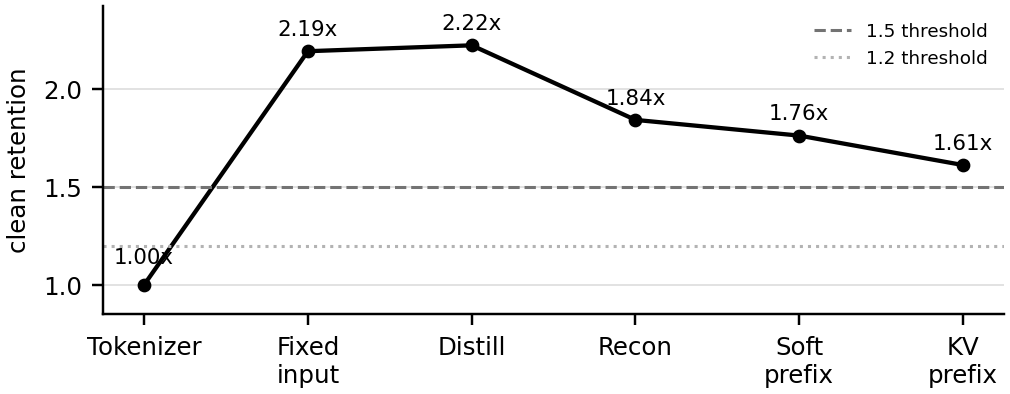
\includegraphics[width=0.78\linewidth]{qwen_diagnostic_ladder.png}
\caption{Clean retention across the \qwen{} diagnostic ladder. Lower is better.}
\label{fig:qwen-ladder}
\end{figure}

Table~\ref{tab:buckets} shows selected bucket losses. The tokenizer baseline remains strongest on clean English, code, tokenizer-stress, Unicode, and multilingual text. The byte adapters are strongest on typo noise. This is the one robust positive signal across phases: when the prompt is corrupted but the target is clean, byte adapters can learn a denoising-style context that degrades less than native tokenized conditioning.

\begin{table}[t]
\centering
\caption{Selected \qwen{} test losses. Lower is better. Byte-derived adapters consistently help typo-noise buckets but remain worse than native tokenization on clean and non-typo stress categories. Multilingual KV-prefix failures are analyzed in Section~8.1.}
\label{tab:buckets}
\small
\setlength{\tabcolsep}{3.3pt}
\begin{tabular}{lrrrrr}
\toprule
Bucket & tokenizer & Phase 2 & Phase 4 & soft prefix & KV prefix \\
 & baseline & best & fixed recon & p64 & p32 all \\
\midrule
clean English & \textbf{0.3089} & 0.6770 & 0.5669 & 0.5441 & 0.4985 \\
code & \textbf{0.3876} & 2.4261 & 2.0058 & 0.7878 & 1.3462 \\
tokenizer stress & \textbf{0.4806} & 3.1706 & 2.8533 & 1.5118 & 1.5969 \\
Unicode stress & \textbf{0.5614} & 3.8226 & 2.3900 & 0.9630 & 0.9809 \\
typo light & 1.3838 & 0.7454 & 0.6416 & 0.5817 & \textbf{0.5167} \\
typo medium & 1.8428 & 0.7786 & 0.6626 & 0.6097 & \textbf{0.5298} \\
typo heavy & 2.8353 & 0.8203 & 0.7749 & 0.6686 & \textbf{0.5986} \\
multilingual zh & \textbf{0.6085} & 4.5419 & 4.7134 & 4.9432 & 11.1217 \\
multilingual ar & \textbf{0.3806} & 3.9973 & 4.4678 & 5.4298 & 10.7503 \\
\bottomrule
\end{tabular}
\end{table}

Deeper injection helps non-typo stress relative to earlier byte variants. Soft prefix p64 reduces code loss from $2.0058$ under fixed reconstruction to $0.7878$, tokenizer-stress from $2.8533$ to $1.5118$, and Unicode from $2.3900$ to $0.9630$. However, these losses remain worse than tokenizer baseline losses of $0.3876$, $0.4806$, and $0.5614$. All-layer KV-prefix gives the best clean loss, but is worse than soft prefix p64 on code and tokenizer-stress, and multilingual losses remain poor.

\subsection{What Each Diagnostic Tells Us}

\paragraph{Fixed Byte Patches Are Insufficient.}
The Phase 2 input-layer adapter confirms engineering feasibility: gradients flow through \texttt{inputs\_embeds}, LM trainable parameters remain zero, and checksum drift is zero. But its best clean retention is only $2.19\times$, with severe degradation on Unicode, code, multilingual, and tokenizer-stress buckets.

\paragraph{Embedding Alignment Is Not Enough.}
Projection alignment works as an auxiliary objective: distillation loss drops from $0.9583$ to $0.0637$ for $L=32$ and from $0.9654$ to $0.0752$ for $L=64$. Downstream LM evaluation does not improve: the $L=32$ distill-then-LM run has $2.22\times$ clean retention. Matching token embeddings geometrically is therefore not enough.

\paragraph{Token Identity Is Learnable, but Not Sufficient.}
Token reconstruction is stronger than embedding alignment. Fixed reconstruction reaches validation clean top-1 accuracy $0.8669$, and oracle-boundary reconstruction reaches $0.9945$. Yet downstream clean retention remains poor: fixed reconstruction improves to $1.84\times$, while oracle-boundary reconstruction is $2.20\times$. Boundary and identity errors are real bottlenecks, but not the only bottlenecks.

\paragraph{Deeper Injection Helps, but Not Enough.}
Soft prefix and KV-prefix variants test whether the frozen model needs byte information as attention context rather than replacement input embeddings. The answer is partially yes: soft prefix p64 improves code, Unicode, and tokenizer-stress losses over input-layer variants, and all-layer KV-prefix gives the best clean retention, $1.61\times$. But neither reaches $1.5\times$ clean retention, and neither beats the tokenizer baseline on non-typo stress buckets.

\section{Is the Typo Gain Just Preprocessing?}

A natural objection is that the typo-noise gains may be explained by simple input cleanup. We therefore evaluate deterministic preprocessing baselines on the native tokenizer path. Each transform is applied only to the input side; the target text and target-token scoring stay unchanged. Table~\ref{tab:preprocess} summarizes the main controls.

\begin{table}[t]
\centering
\caption{Deterministic preprocessing controls on \qwen{} tokenizer baseline. Conservative transforms do not explain the typo gains. Strong cleanup improves typo loss but damages clean loss. The oracle row uses the clean prompt for typo examples and is not deployable.}
\label{tab:preprocess}
\small
\setlength{\tabcolsep}{4pt}
\begin{tabular}{lrrrrr}
\toprule
Mode & changed frac. & clean & typo L & typo M & typo H \\
\midrule
raw tokenizer & 0.000 & 0.3089 & 1.3838 & 1.8428 & 2.8353 \\
NFC & 0.015 & 0.3089 & 1.3838 & 1.8428 & 2.8353 \\
whitespace cleanup & 0.112 & 0.3089 & 1.3518 & 1.8257 & 2.8137 \\
repeat squeeze & 0.039 & 0.3089 & 1.3835 & 1.8429 & 2.8189 \\
casefold & 0.693 & 0.6028 & 1.0721 & 1.4980 & 2.4380 \\
typo cleanup & 0.709 & 0.6028 & 1.0748 & 1.5098 & 2.4155 \\
oracle clean typo & 0.296 & 0.3089 & 0.3039 & 0.3039 & 0.3039 \\
\midrule
soft prefix p64 & -- & 0.5441 & 0.5817 & 0.6097 & 0.6686 \\
KV prefix p32 all & -- & 0.4985 & 0.5167 & 0.5298 & 0.5986 \\
\bottomrule
\end{tabular}
\end{table}

The result is mixed in a useful way. Conservative cleanup, such as Unicode NFC normalization, whitespace cleanup, and repeated-character squeezing, barely changes the typo buckets. Stronger cleanup, such as case folding and our combined typo cleanup, improves typo loss but roughly doubles clean loss from $0.3089$ to $0.6028$. Byte adapters remain much better on typo loss than these deterministic transforms. The oracle row shows that the paired task can be easy if the clean prompt is known, but this is an upper bound, not a deployable baseline. The typo signal is therefore real, but narrow: it does not imply broad tokenizer-free superiority.

\section{Mechanism Analysis}

\subsection{Fragmentation Correlates with Loss, but Does Not Explain Everything}

Tokenizer-unfriendly strings often produce longer token sequences. We measure several fragmentation proxies on the fixed test set: input byte length, input token length, tokens per byte, and bytes per token. We then correlate these with tokenizer loss and with byte-adapter gain over the tokenizer baseline.

Table~\ref{tab:frag} gives selected correlations. Input token length has a strong Pearson correlation with tokenizer loss ($0.669$) but a much weaker Spearman correlation ($0.214$), meaning length is useful but not a complete ranking signal. Tokens per byte has a smaller Pearson correlation ($0.227$) and a moderate Spearman correlation ($0.334$). Byte adapters gain more on longer tokenized inputs, with Spearman correlations of $0.459$ for soft prefix p64 and $0.477$ for KV-prefix p32 all-layer. Still, high fragmentation is not enough to predict success. Multilingual buckets are highly problematic for byte adapters even though byte input should, in principle, avoid vocabulary coverage issues. Figure~\ref{fig:fragmentation} summarizes this bucket-level pattern.

\begin{table}[t]
\centering
\caption{Selected fragmentation correlations over 2028 \qwen{} test samples. Fragmentation helps explain tokenizer stress, but it does not fully explain where byte adapters work.}
\label{tab:frag}
\small
\begin{tabular}{llrr}
\toprule
Predictor & outcome & Pearson & Spearman \\
\midrule
input token length & tokenizer loss & 0.669 & 0.214 \\
tokens per byte & tokenizer loss & 0.227 & 0.334 \\
bytes per token & tokenizer loss & -0.319 & -0.334 \\
input token length & soft prefix gain & 0.276 & 0.459 \\
input token length & KV-prefix gain & 0.349 & 0.477 \\
\bottomrule
\end{tabular}
\end{table}

\begin{figure}[t]
\centering
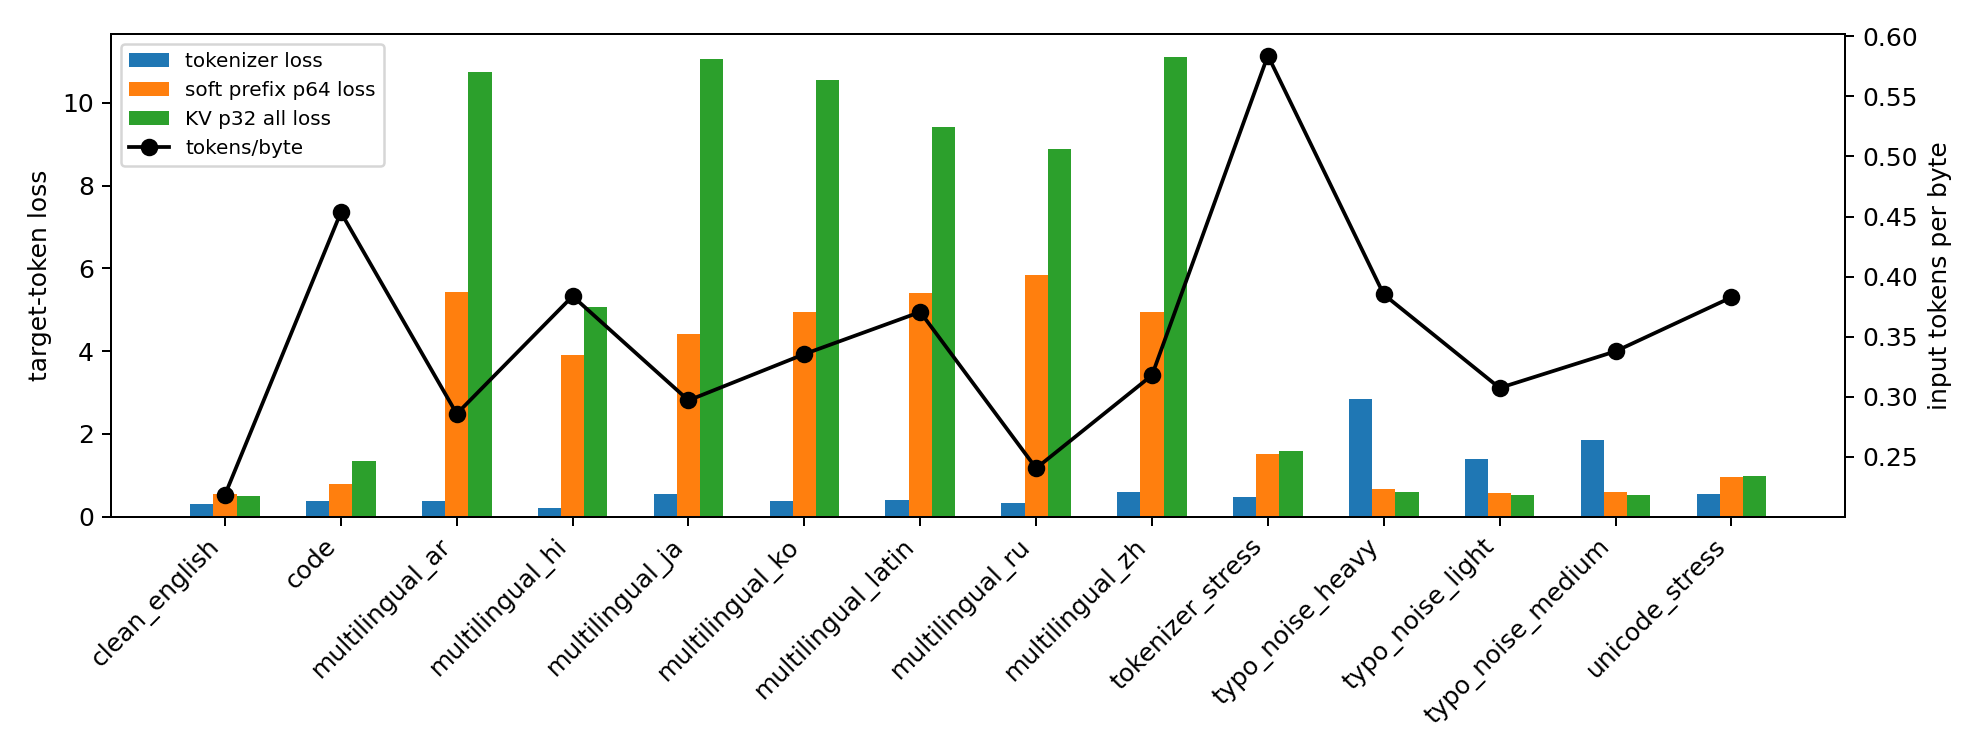
\includegraphics[width=0.92\linewidth]{bucket_loss_and_fragmentation.png}
\caption{Bucket-level loss and fragmentation view. Longer tokenized inputs are often harder for the tokenizer baseline, but byte adapters do not automatically solve all high-fragmentation buckets.}
\label{fig:fragmentation}
\end{figure}

\subsection{Interpretation}

The diagnostics narrow the failure mode. Embedding alignment, oracle token boundaries, and deeper prefix injection each help only partially. If the issue were only embedding geometry, boundary segmentation, or shallow input injection, one of these interventions should have closed the clean-retention gap. None did.

Our interpretation is that frozen tokenizer-based language models depend on several tokenizer-created conventions at once. Native token embeddings carry local text content, but the model also expects familiar token units, familiar boundary lengths, familiar position steps, and familiar attention patterns. A small byte adapter trained after the fact can learn useful robust cues, especially for typo-noise denoising, but it does not recreate the full input interface.

The multilingual failures are especially important. They do not show that byte modeling is bad for multilingual text. Byte-trained models are often attractive precisely because they avoid vocabulary coverage problems. Instead, they show that our small adapters do not compress non-Latin byte sequences into context that frozen Qwen can use as well as its native tokenizer. This may reflect longer byte sequences, limited adapter training coverage, and the fact that Qwen's own tokenizer already provides strong script-specific units.

\section{Cross-Model Replication}

To test whether the Qwen result is model-family specific, we run selected replications on two additional frozen models. This is not a full rerun of the entire diagnostic ladder. It is a focused check of the best later-stage interfaces: soft prefix p64 and all-layer KV-prefix p32.

The first replication uses \qwena{}. This keeps the tokenizer family and cache API close to the primary model, reducing engineering confounds while testing a larger frozen Qwen2.5 model. The native \qwena{} tokenizer clean loss is $0.3274$. Soft prefix p64 improves with longer training, from $6.22\times$ clean retention at 2000 steps to $2.73\times$ at 8000 steps, but remains far above the $1.5\times$ threshold. All-layer KV-prefix is the best selected \qwena{} run, with $2.52\times$ clean retention. It beats the tokenizer baseline only on medium and heavy typo noise.

The second replication uses \tinyllama{}, which changes the tokenizer and model family. Here the result is different. The native tokenizer clean loss is $0.6026$. Soft prefix p64 reaches $1.26\times$ clean retention and beats the tokenizer baseline on all three typo buckets. All-layer KV-prefix p32 is much stronger: across three seeds, its mean clean retention is $0.63\times$, and the three seed values are $0.69$, $0.66$, and $0.55$. The three-seed mean beats the tokenizer baseline on clean English, all typo buckets, and Unicode stress. It still loses on tokenizer-stress strings and fails badly on multilingual buckets. A target-only sanity baseline has clean loss $5.4014$, and a learned constant KV-prefix that never reads input bytes has clean loss $0.8907$. These controls show that target-side prediction and generic soft prompting do not explain the full TinyLlama KV result.

\begin{table}[t]
\centering
\caption{Selected cross-model replication. \qwena{} follows the Qwen negative pattern, while \tinyllama{} KV-prefix is stronger but still fails on tokenizer-stress and multilingual inputs.}
\label{tab:qwen15}
\footnotesize
\setlength{\tabcolsep}{2.4pt}
\begin{tabular}{llrrrp{2.6cm}}
\toprule
Model & run & clean loss & retention & steps & wins \\
\midrule
\qwena{} & tokenizer & 0.3274 & 1.00 & 0 & -- \\
\qwena{} & prefix p64 & 0.8927 & 2.73 & 8000 & typo H \\
\qwena{} & KV p32 all & 0.8245 & 2.52 & 2000 & typo M/H \\
\midrule
\tinyllama{} & target-only & 5.4014 & 8.96 & 0 & none \\
\tinyllama{} & tokenizer & 0.6026 & 1.00 & 0 & -- \\
\tinyllama{} & prefix p64 & 0.7609 & 1.26 & 2000 & typo L/M/H \\
\tinyllama{} & constant KV & 0.8907 & 1.48 & 2000 & typo L/M/H \\
\tinyllama{} & KV p32 all & 0.3811 & 0.63 & 2000 & clean; typo L/M/H; Unicode \\
\bottomrule
\end{tabular}
\end{table}

\begin{table}[t]
\centering
\caption{\tinyllama{} bucket-level results. Byte KV p32 all-layer values are means over three seeds. Constant KV is a learned prefix that does not read input bytes. Positive byte gain means lower loss than the tokenizer baseline; negative gain means degradation.}
\label{tab:tinyllama-buckets}
\footnotesize
\setlength{\tabcolsep}{3.2pt}
\begin{tabular}{lrrrr}
\toprule
Bucket & tokenizer & constant KV & byte KV & byte gain \\
\midrule
clean English & 0.6026 & 0.8907 & \textbf{0.3811} & 36.8\% \\
typo light & 1.4080 & 0.8869 & \textbf{0.3823} & 72.8\% \\
typo medium & 1.7133 & 0.8870 & \textbf{0.3930} & 77.1\% \\
typo heavy & 2.5426 & 0.8870 & \textbf{0.4313} & 83.0\% \\
Unicode stress & 0.7818 & 1.9301 & \textbf{0.6620} & 15.3\% \\
code & \textbf{0.6087} & 1.5146 & 0.7778 & -27.8\% \\
tokenizer stress & \textbf{0.6057} & 2.1189 & 1.2281 & -102.8\% \\
multilingual zh & \textbf{0.5049} & 4.3321 & 10.7154 & -2022.3\% \\
multilingual ar & \textbf{0.4396} & 4.4745 & 11.1403 & -2434.3\% \\
\bottomrule
\end{tabular}
\end{table}

\subsection{Why the TinyLlama Result Is Not a Contradiction}

The TinyLlama result changes the interpretation, but it does not overturn the main caution. The Qwen experiments show that byte adapters are not reliable drop-in replacements for native tokenization. Even all-layer KV-prefix misses the clean-retention threshold and never beats the tokenizer baseline outside typo noise. TinyLlama shows the other side of the boundary: the failure is not universal, and a frozen model can sometimes use byte-derived KV memory better than its tokenized prompt.

We do not identify a single cause for the TinyLlama-Qwen gap. Two clues are useful, but neither is a complete explanation. First, TinyLlama's native tokenizer baseline is weaker on this benchmark, with clean loss $0.6026$ rather than Qwen2.5-0.5B's $0.3089$. Second, TinyLlama tokenizes the same test inputs more densely. Its input tokens per byte are higher on clean text ($0.241$ vs. $0.218$), Unicode stress ($0.493$ vs. $0.383$), code ($0.533$ vs. $0.453$), tokenizer-stress strings ($0.700$ vs. $0.584$), Chinese ($0.550$ vs. $0.318$), and Arabic ($0.547$ vs. $0.286$). This suggests that TinyLlama may leave more room for byte-conditioned KV memory on several buckets. Yet fragmentation is not enough: TinyLlama's multilingual inputs are also highly fragmented, but native tokenizer loss remains low and byte KV fails badly.

The training curves rule out another simple explanation. All-layer KV-prefix training optimizes for both models: Qwen2.5-0.5B drops from training loss $8.61$ to $0.25$, and the three TinyLlama seeds drop from $10.36/11.28/10.76$ to $0.21/0.30/0.22$. Thus the Qwen failure is not simply a stalled optimizer. The difference appears in validation and test behavior. TinyLlama reaches validation clean losses between $0.30$ and $0.39$, while Qwen2.5-0.5B reaches $0.468$. A TinyLlama constant KV-prefix, shared across examples and not conditioned on input bytes, plateaus at validation clean loss $0.824$ and test clean loss $0.8907$. So the TinyLlama gain is not just an easy target suffix, generic soft prompting, or optimizer success.

We also compare each learned byte KV cache with the native cache produced by tokenized prompts. This does not support the simple idea that TinyLlama works because its byte KV tensors are globally closer to native KV tensors. Qwen's byte-to-native key/value RMS ratios are $0.69/3.12$, while TinyLlama's are $1.61/19.26$. TinyLlama has only slightly higher mean-vector cosine ($0.071/0.039$ for key/value, versus Qwen's $0.021/-0.032$). The result points instead to a sensitivity difference: TinyLlama can use some high-magnitude byte-derived prefix memory, even though that memory is not a faithful copy of its native prompt cache.

The multilingual failures make the limit concrete. The all-layer KV adapters are trained on clean English, typo noise, Unicode, code, and tokenizer-stress buckets, but not on multilingual buckets. In the worst held-out cases, native tokenization has low loss on short non-Latin sentences while byte KV fails catastrophically. For Arabic examples of 83 bytes, Qwen/TinyLlama use 23/43 input tokens and have tokenizer losses around $0.30$--$0.43$, but byte KV losses around $11$--$12$. Chinese examples of 58--64 bytes show the same pattern: 18--19 Qwen tokens, 31--33 TinyLlama tokens, tokenizer loss around $0.46$--$0.63$, and byte KV loss around $11$--$12$. The problem is therefore not simply sequence length. The adapter learns useful byte cues for trained buckets, but it does not acquire the script-specific input structure that the native tokenizers inherit from pretraining. The safest conclusion is model- and bucket-dependent: byte-derived attention memory can be useful, but it is not yet a dependable replacement for native tokenization.

\section{Related Work}

\paragraph{Subword Tokenization.}
Subword tokenizers such as byte-pair encoding, WordPiece, and SentencePiece are widely used because they balance vocabulary size and open-vocabulary coverage \cite{devlin2019bert,kudo2018sentencepiece,schuster2012japanese,sennrich2016neural}. Prior work has shown that tokenization choices affect robustness, fairness, multilingual efficiency, and downstream performance, and that stochastic subword variants can improve robustness in some settings \cite{bostrom2020bytepair,kudo2018subword,mielke2021between,provilkov2020bpedropout,rust2021good}. \bb{} focuses on a complementary question: whether an already-tokenized language model can be retrofitted with a byte-based input side while keeping the model frozen.

\paragraph{Byte and Character-Level Language Models.}
ByT5 removes text preprocessing and operates directly on UTF-8 bytes, improving robustness and multilingual coverage in an encoder-decoder setting \cite{xue2022byt5}. CANINE models Unicode characters with downsampling and upsampling to reduce sequence length \cite{clark2022canine}. Charformer learns gradient-based subword tokenization within the model \cite{tay2022charformer}. MEGABYTE uses multiscale byte modeling with patch-level structure for long byte sequences \cite{yu2023megabyte}. These systems differ from \bb{} because they train architectures for byte or character inputs, whereas we freeze an existing tokenizer-based model and train only an external input adapter.

\paragraph{Parameter-Efficient Frozen-Model Adaptation.}
Prompt tuning, prefix tuning, adapters, and LoRA demonstrate that frozen or mostly frozen language models can be steered by small trainable modules \cite{houlsby2019adapter,hu2022lora,lester2021prompttuning,li2021prefixtuning}. Our soft-prefix and KV-prefix experiments borrow this intuition, but the task is different. Standard prompt or prefix tuning usually keeps the model's native tokenizer on the input text and learns task-conditioning vectors. \bb{} instead asks the trainable module to encode the raw input string itself from bytes. It must provide the content that a tokenized prompt would normally provide, not only a task instruction. This distinction explains why a constant prefix is an important control: it tests generic soft-prompt benefit separately from input-conditioned byte memory.

\paragraph{Diagnostic Negative and Mixed Results.}
\bb{} is closest in spirit to diagnostic work on when a tempting modeling shortcut fails or works only under narrow conditions. The contribution is not a new universal byte architecture. It is a controlled comparison showing which explanations are insufficient: embedding alignment alone, oracle boundary reconstruction alone, and deeper prefix injection alone do not make Qwen2.5 byte adapters reliable. The TinyLlama result adds the complementary lesson that the failure is not universal. This makes the study a boundary-finding result rather than a simple method paper.

\section{Limitations}

This study is scoped to Qwen2.5 and TinyLlama models, small adapters, a single-GPU environment, and a synthetic or curated stress benchmark. The benchmark is designed for controlled diagnosis, not for estimating real-world frequency or user impact. The typo gains should therefore be read as evidence that byte adapters can use noisy byte-level cues under a paired benchmark, not as a deployment claim about all user typos. Real user text may contain different noise patterns, longer contexts, mixed tasks, and domain-specific conventions.

We do not claim that all byte interfaces for all frozen language models must fail, or that the TinyLlama success will transfer to other model families. We also do not eliminate the target-side tokenizer: supervision and output scoring use each model's native target tokens to make comparisons fair. The study has not tested many tokenizer families, substantially larger adapters, long training schedules beyond the selected \qwena{} check, contrastive pretraining with hard negatives, or partial LM finetuning.

The oracle-boundary reconstruction experiments use tokenizer-derived boundaries and therefore are diagnostic upper bounds, not tokenizer-free systems. KV-prefix experiments use a practical cache construction for the installed Transformers version; first-$N$-layer variants use zero K/V tensors for non-injected layers to maintain cache length consistency, which may not be optimal.

\section{Conclusion}

\bb{} asks whether a small input-side byte adapter can replace or augment native tokenized input for a frozen tokenizer-based language model. The answer is mixed. Under Qwen2.5, byte adapters produce a consistent typo-noise robustness signal and deeper injection improves several stress categories, but clean retention remains too poor and native tokenization continues to dominate non-typo stress buckets. Under \tinyllama{}, all-layer KV-prefix injection is much stronger and beats native tokenization on clean, typo, and Unicode buckets, but still fails on tokenizer-stress and multilingual inputs. Deterministic preprocessing controls do not explain away the typo signal, and fragmentation analysis shows only a partial mechanism. Future byte-interface retrofitting methods should treat model family, tokenizer family, and input bucket as central variables rather than assuming that one byte adapter interface will replace native tokenization everywhere.

\subsubsection*{Reproducibility statement.}
All experiments save configuration files, environment metadata, training metrics, summaries, checkpoints, and per-bucket evaluation outputs. The Phase 2 train, validation, and test manifests are reused unchanged across all later diagnostic and control experiments. In all reported LM runs, the frozen model trainable parameter count is zero and the frozen checksum delta is zero.

\bibliographystyle{splncs04}
\bibliography{references}

\end{document}
